\documentclass[answers]{exam}
\usepackage{texPreamble}
\usepackage{relsize}
\usepackage{tabularx}
\extraheadheight{0.25in}
\extrafootheight{1.0in}
\extrawidth{1in}
% ----------------------------------------------------------------
\begin{document}
\section{JIT 4.3: Power Functions}
  \begin{defn*}
    Functions of the form $f(x)=x^r$, where $r$ is a constant, are called \textbf{power functions}.
  \end{defn*}
  \begin{enumerate}[label=]
    \item 
      \begin{minipage}{0.45\linewidth}
        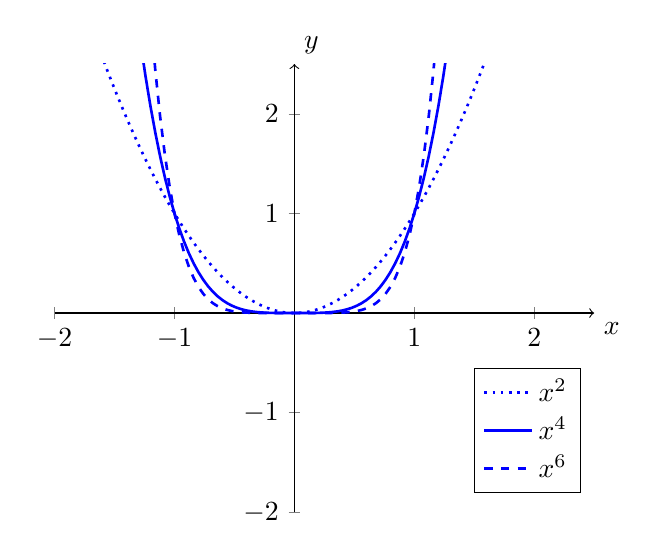
\begin{tikzpicture}[scale=1.0]
          \begin{axis}[
            axis lines=center,
            axis line style={->},
            xmin=-2, xmax=2.5,
            ymin=-2, ymax=2.5,
            xtick={-2,-1,...,2},
            ytick={-2,-1,...,2},
            xlabel=$x$, xlabel style={at={(ticklabel* cs:1)},anchor=north west},
            ylabel=$y$, ylabel style={at={(ticklabel* cs:1)},anchor=south west},
            legend style={at={(axis cs:1.5,-0.55)},anchor=north west},
            every axis plot/.append style={line width=0.95pt}
            ]
            \addplot[domain=-2:2,blue, samples = 101, dotted] {x^2};
              \addlegendentry{$x^2$};
            \addplot[domain=-2:2,blue, samples = 101] {x^4};
              \addlegendentry{$x^4$};
            \addplot[domain=-2:2,blue, samples = 101, dashed] {x^6};
              \addlegendentry{$x^6$};
          \end{axis}
        \end{tikzpicture}
      \end{minipage}%
      \begin{minipage}{0.55\linewidth}
        \begin{enumerate}[label=-]
          \item 
            These are \textbf{even} functions

            $f(-x)=f(x)$
            
          \item 
            Symmetry about the $y$-axis
            
            $(-x,y),\ (x,y)$
        \end{enumerate}
        \vspace*{100pt}
      \end{minipage}

  
      \vspace*{\stretch{1}}
    \item 
      \begin{minipage}{0.45\linewidth}
        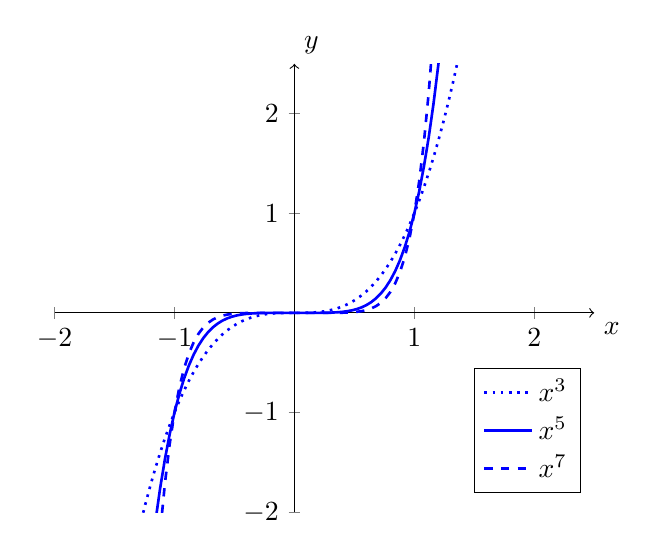
\begin{tikzpicture}[scale=1.0]
          \begin{axis}[
            axis lines=center,
            axis line style={->},
            xmin=-2, xmax=2.5,
            ymin=-2, ymax=2.5,
            xtick={-2,-1,...,2},
            ytick={-2,-1,...,2},
            xlabel=$x$, xlabel style={at={(ticklabel* cs:1)},anchor=north west},
            ylabel=$y$, ylabel style={at={(ticklabel* cs:1)},anchor=south west},
            legend style={at={(axis cs:1.5,-0.55)},anchor=north west},
            every axis plot/.append style={line width=0.95pt}
            ]
            \addplot[domain=-2:2,blue, samples = 101, dotted] {x^3};
              \addlegendentry{$x^3$};
            \addplot[domain=-2:2,blue, samples = 101] {x^5};
              \addlegendentry{$x^5$};
            \addplot[domain=-2:2,blue, samples = 101, dashed] {x^7};
              \addlegendentry{$x^7$};
          \end{axis}
        \end{tikzpicture}
      \end{minipage}%
      \begin{minipage}{0.55\linewidth}
        \begin{enumerate}[label=-]
          \item 
            These are \textbf{odd} functions

            $f(-x)=-f(x)$
          \item 
            Symmetry about the origin
            
            $(-x,-y),\ (x,y)$
        \end{enumerate}
        \vspace*{100pt}
      \end{minipage}

      \vspace*{\stretch{0.75}}
      \pagebreak
      
      \item 
      \begin{minipage}{0.5\linewidth}
        \begin{tikzpicture}[scale=1.0]
          \begin{axis}[
            axis lines=center,
            axis line style={->},
            xmin=-2, xmax=2.5,
            ymin=-1.5, ymax=1.75,
            xtick={-2,-1,...,2},
            ytick={-2,-1,...,2},
            xlabel=$x$, xlabel style={at={(ticklabel* cs:1)},anchor=north west},
            ylabel=$y$, ylabel style={at={(ticklabel* cs:1)},anchor=south west},
            legend style={at={(axis cs:1.5,-0.55)},anchor=north west},
            every axis plot/.append style={line width=0.95pt}
            ]
            \addplot[domain=0:2.5,blue, samples = 101, dotted] {x^0.5};
              \addlegendentry{$x^{\sfrac12}$};
            \addplot[domain=0:2.5,blue, samples = 101] {x^0.25};
              \addlegendentry{$x^{\sfrac14}$};
            \addplot[domain=0:2.5,blue, samples = 101, dashed] {x^0.16};
              \addlegendentry{$x^{\sfrac16}$};
          \end{axis}
        \end{tikzpicture}
      \end{minipage}%
      \begin{minipage}{0.5\linewidth}
        \begin{tikzpicture}[scale=1.0]
          \begin{axis}[
            axis lines=center,
            axis line style={->},
            xmin=-2, xmax=2.5,
            ymin=-1.5, ymax=1.75,
            xtick={-2,-1,...,2},
            ytick={-2,-1,...,2},
            xlabel=$x$, xlabel style={at={(ticklabel* cs:1)},anchor=north west},
            ylabel=$y$, ylabel style={at={(ticklabel* cs:1)},anchor=south west},
            legend style={at={(axis cs:1.5,-0.55)},anchor=north west},
            every axis plot/.append style={line width=0.9pt}
            ]
            \def\g(#1){(#1)}
            \def\f(#1,#2){(\g(#1))/abs(\g(#1))*(abs(\g(#1)))^(#2)};
            \addplot[domain=-2:2,blue, samples = 501, dotted] {\f(\x,1/3)};
              \addlegendentry{$x^{\sfrac13}$};
            \addplot[domain=-2:2,blue, samples = 501] {\f(\x,1/5)};
              \addlegendentry{$x^{\sfrac15}$};
            \addplot[domain=-2:2,blue, samples = 501, dashed] {\f(\x,1/7)};
              \addlegendentry{$x^{\sfrac17}$};
          \end{axis}
        \end{tikzpicture}
      \end{minipage}

  
      \vspace*{\stretch{1}}

      \begin{center}
        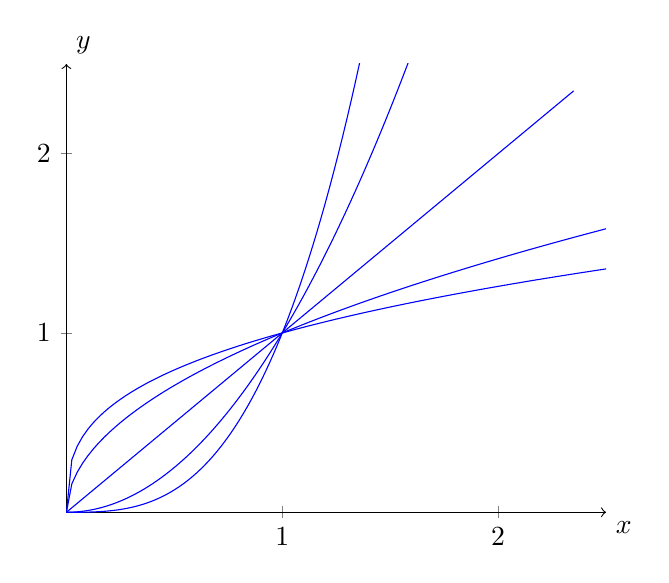
\begin{tikzpicture}[scale=1.0]
          \begin{axis}[
            axis lines=center,
            axis line style={->},
            xmin=0, xmax=2.5,
            ymin=0, ymax=2.5,
            xtick={-2,-1,...,2},
            ytick={-2,-1,...,2},
            xlabel=$x$, xlabel style={at={(ticklabel* cs:1)},anchor=north west},
            ylabel=$y$, ylabel style={at={(ticklabel* cs:1)},anchor=south west},
            legend style={at={(axis cs:1.5,-0.55)},anchor=north west},
            %every axis plot/.append style={line width=0.95pt}
            ]
            \addplot[domain=0:2.5,blue, samples = 101] {x^(1/3)};
            \addplot[domain=0:2.5,blue, samples = 101] {x^(1/2)};
            \addplot[domain=0:2.35,blue, samples = 101] {x^1};
            \addplot[domain=0:2,blue, samples = 101] {x^2};
            \addplot[domain=0:2,blue, samples = 101] {x^3};
          \end{axis}
        \end{tikzpicture}
      \end{center}

      \pagebreak      
      \item 
      \begin{minipage}{0.5\linewidth}
        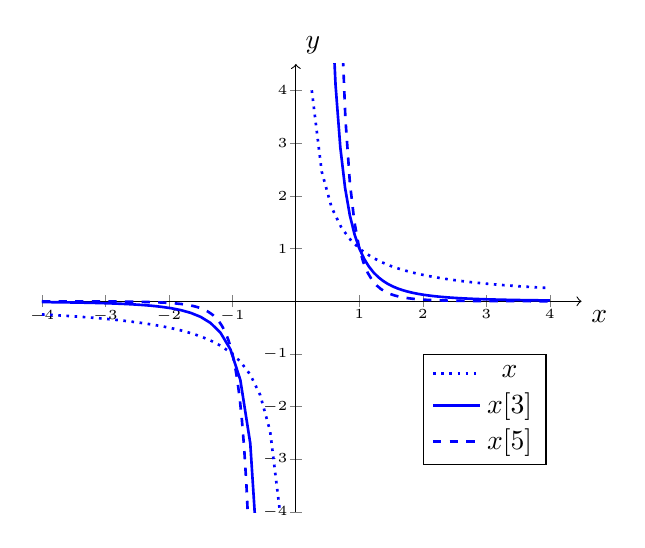
\begin{tikzpicture}[scale=1.0]
          \begin{axis}[
            axis lines=center,
            axis line style={->},
            xmin=-4, xmax=4.5,
            ymin=-4, ymax=4.5,
            xtick={-4,-3,...,4},
            ytick={-4,-3,...,4},
            ticklabel style={font=\tiny, inner sep=0.75pt},
            xlabel=$x$, xlabel style={at={(ticklabel* cs:1)},anchor=north west},
            ylabel=$y$, ylabel style={at={(ticklabel* cs:1)},anchor=south west},
            legend style={at={(axis cs:2,-1)},anchor=north west},
            every axis plot/.append style={line width=0.95pt}
            ]
            \addplot[unbounded coords=jump,domain=-4:-0.25,blue, dotted] {1/x};
              \addlegendentry{$x\inv$};
            \addplot[unbounded coords=jump,domain=-4:-0.25,blue] {1/x^3};
              \addlegendentry{$x\inv[3]$};
            \addplot[unbounded coords=jump,domain=-4:-0.5,blue, dashed, samples=101] {1/x^5};
              \addlegendentry{$x\inv[5]$};
            \addplot[unbounded coords=jump,domain=0.25:4,blue, dotted] {1/x};
            \addplot[unbounded coords=jump,domain=0.25:4,blue, samples = 51] {1/x^3};
            \addplot[unbounded coords=jump,domain=0.5:4,blue, samples = 51, dashed] {1/x^5};
          \end{axis}
        \end{tikzpicture}
      \end{minipage}%
      \begin{minipage}{0.5\linewidth}
        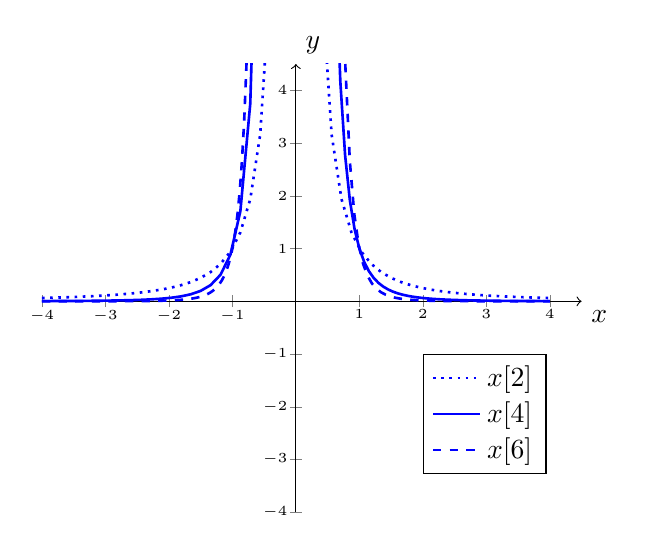
\begin{tikzpicture}[scale=1.0]
          \begin{axis}[
            axis lines=center,
            axis line style={->},
            xmin=-4, xmax=4.5,
            ymin=-4, ymax=4.5,
            xtick={-4,-3,...,4},
            ytick={-4,-3,...,4},
            ticklabel style={font=\tiny, inner sep=0.75pt},
            xlabel=$x$, xlabel style={at={(ticklabel* cs:1)},anchor=north west},
            ylabel=$y$, ylabel style={at={(ticklabel* cs:1)},anchor=south west},
            legend style={at={(axis cs:2,-1)},anchor=north west},
            every axis plot/.append style={line width=0.95pt}
            ]
            \addplot[unbounded coords=jump,domain=-4:-0.25,blue, dotted] {1/x^2};
              \addlegendentry{$x\inv[2]$};
            \addplot[unbounded coords=jump,domain=-4:-0.25,blue] {1/x^4};
              \addlegendentry{$x\inv[4]$};
            \addplot[unbounded coords=jump,domain=-4:-0.5,blue, dashed, samples=101] {1/x^6};
              \addlegendentry{$x\inv[6]$};
            \addplot[unbounded coords=jump,domain=0.25:4,blue, dotted] {1/x^2};
            \addplot[unbounded coords=jump,domain=0.25:4,blue, samples = 51] {1/x^4};
            \addplot[unbounded coords=jump,domain=0.5:4,blue, samples = 51, dashed] {1/x^6};
          \end{axis}
        \end{tikzpicture}
      \end{minipage}

      \vspace*{\stretch{1}}
      \begin{ex*}
        Determine if the following functions are symmetric about the $y$-axis, $x$-axis or the origin.
        \begin{enumerate}
          \item 
            $f(x)=3x^5+2x^3-x$\\[\stretch{0.5}]
          \item 
            $f(x)=2\abs{x}$\\[\stretch{0.5}]
          \item 
            $x^3-y^5=0$\\[\stretch{0.5}]
          \item 
            $f(x)=x\abs{x}$\\[\stretch{0.5}]
        \end{enumerate}
      \end{ex*}
    \end{enumerate}
  \pagebreak
  
\end{document}